\section{Ramseyova teorie}
Ramseyova teorie zkoumá především výskyt zajímavých struktur na velmi velkých grafech. Ramseyových vět existuje hned několik, začneme ovšem jinou extremální větou a to Turánovou. Hlavními výsledky v Ramseyově teorii jsou Hales-Jewett a Van der Waerdenova věta.

\subsection{Turánova věta}

\df Turánův graf $T(n,r)$ {\it je graf na $n$ vrcholech, které byly rozděleny do $r$ skupin, jejichž velikost se liší nejvýš o 1. Hrana vede mezi každými dvěma vrcholy, které nejsou ve stejné skupině.}

Turánovy grafy jsou pokus o konstrukci hranově extremálních grafů neobsahujících podgraf $K_{r+1}$. Turánova věta nám pak říká, že turánovy grafy mají skutečně maximální možný počet hran.

\vt (Turánova, verze 1) {\it Ze všech grafů na $n$ vrcholech, které neobsahují $K_{r+1}$ jako podgraf má $T(n,r)$ nejvyšší počet hran.}

\vt (Turánova, verze 2) {\it Nechť $G$ je graf na $n$ vrcholech neobsahující $K_{r+1}$ jako podgraf. Pak počet hran $G$ je nejvýš ${r-1\over r}\cdot{n^2\over 2} = \left(1-{1\over r}\right)\cdot{n^2\over 2}$.}

\dk (Turánovy věty): Předpokládejme, že $G$ je graf neobsahující $K_{r+1}$ s
maximálním počtem hran. V první části důkazu ukážeme, že $G$ musí být úplný
$r$-partitní graf, v druhé části že se velikost jednotlivých partit může lišit
nejvýš o 1.

\textbf{Část 1.} Graf $G$ neobsahuje trojici vrcholů $u$, $v$, $w$ tž. hrana
vede pouze mezi $u$ a $v$. To dokážeme tak, že buď smažeme $w$ a zkopírujeme
$u$, nebo smažeme $u$ a $v$ a zkopírujeme dvakrát $w$, čímž dostaneme graf s
více hranami. Z toho plyne, že můžeme vrcholy $G$ rozdělit do tříd ekvivalence
na základě nesousednosti (dva vrcholy jsou ve stejné třídě, když mezi nimi
nevede hrana). Třídy ekvivalence tvoří partity a $G$ je tedy úplný
multipartitní graf. Čím více partit, tím více hran, takže $G$ je úplný
$r$-partitní graf.

\begin{figure}[h]
\centering
\begin{subfigure}{8cm}
\begin{subfigure}{3cm}
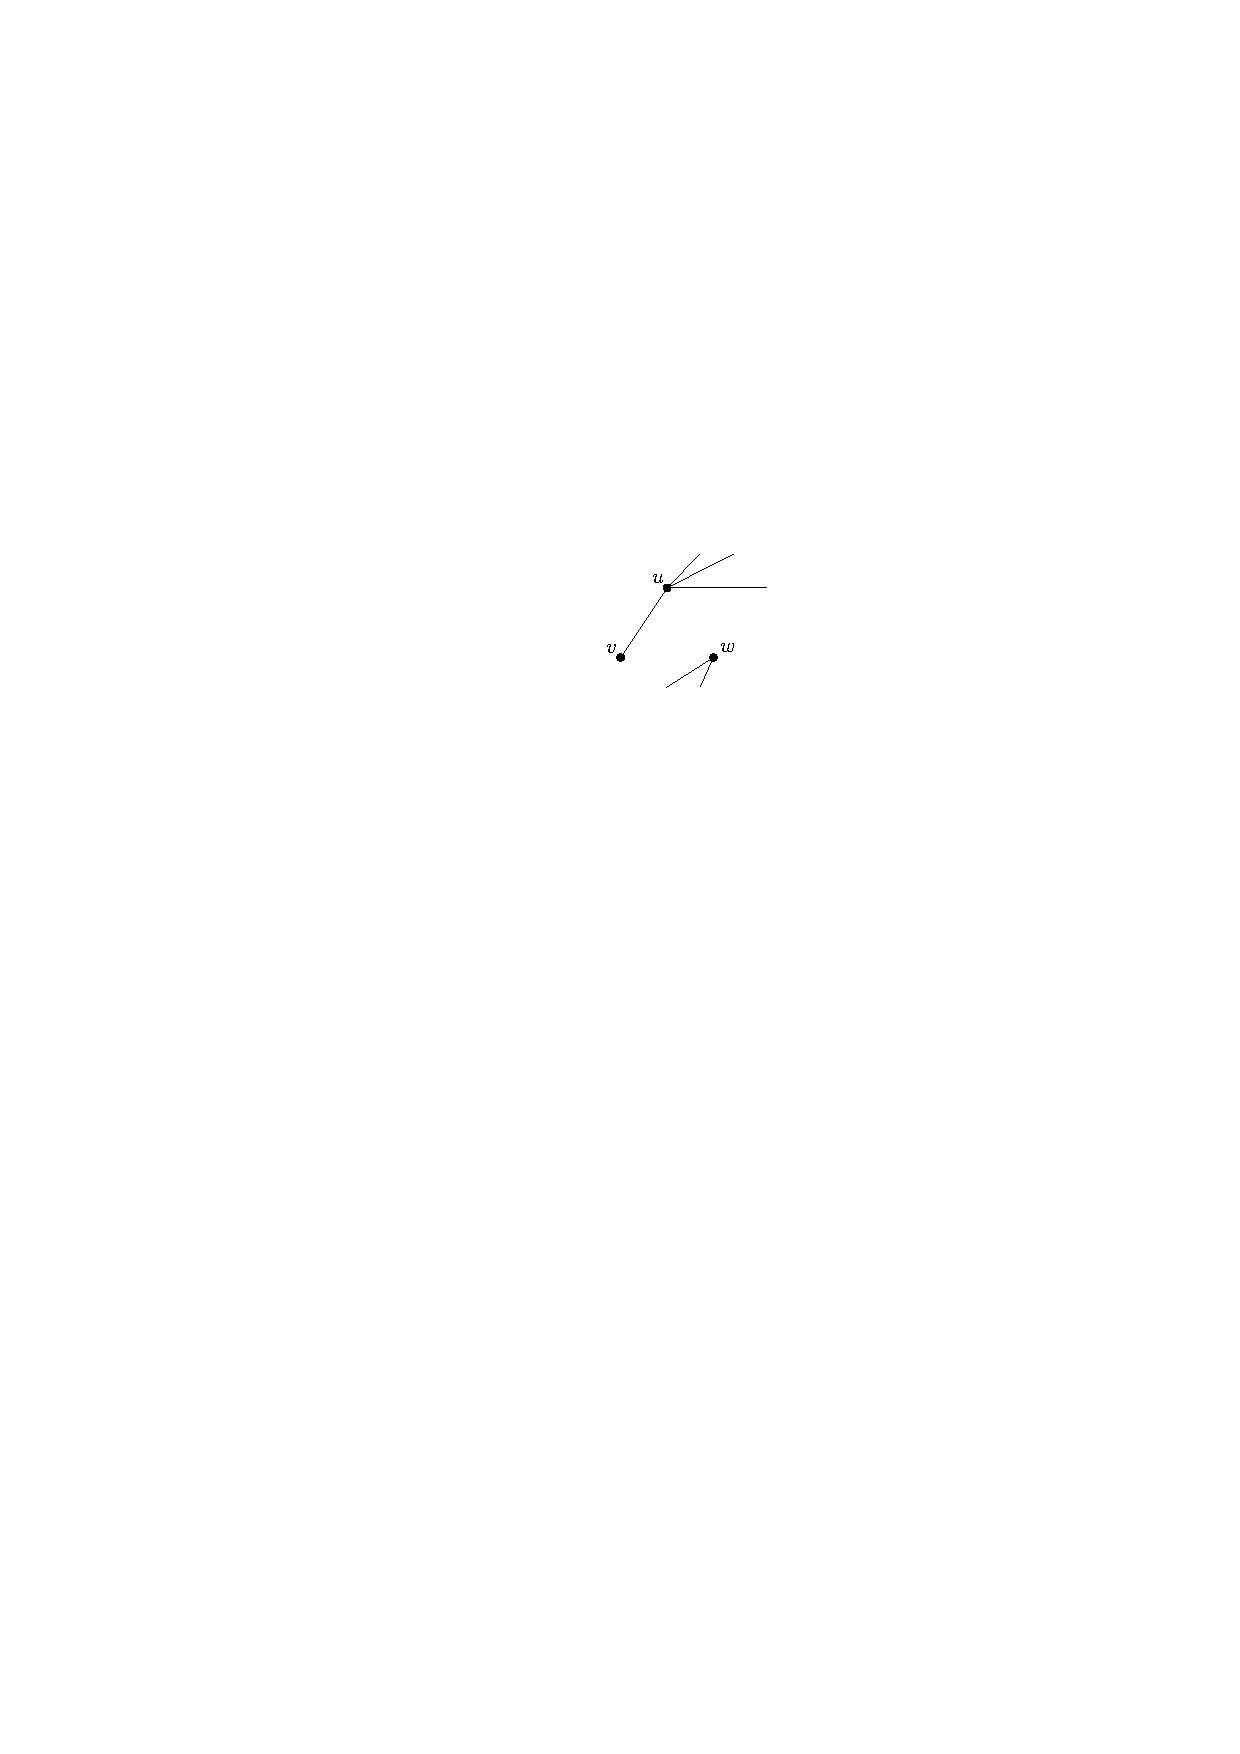
\includegraphics[width=3cm]{img/turan1.pdf}
\end{subfigure}
\hspace{0.5cm}$\Rightarrow$\hspace{0.5cm}
\begin{subfigure}{3cm}
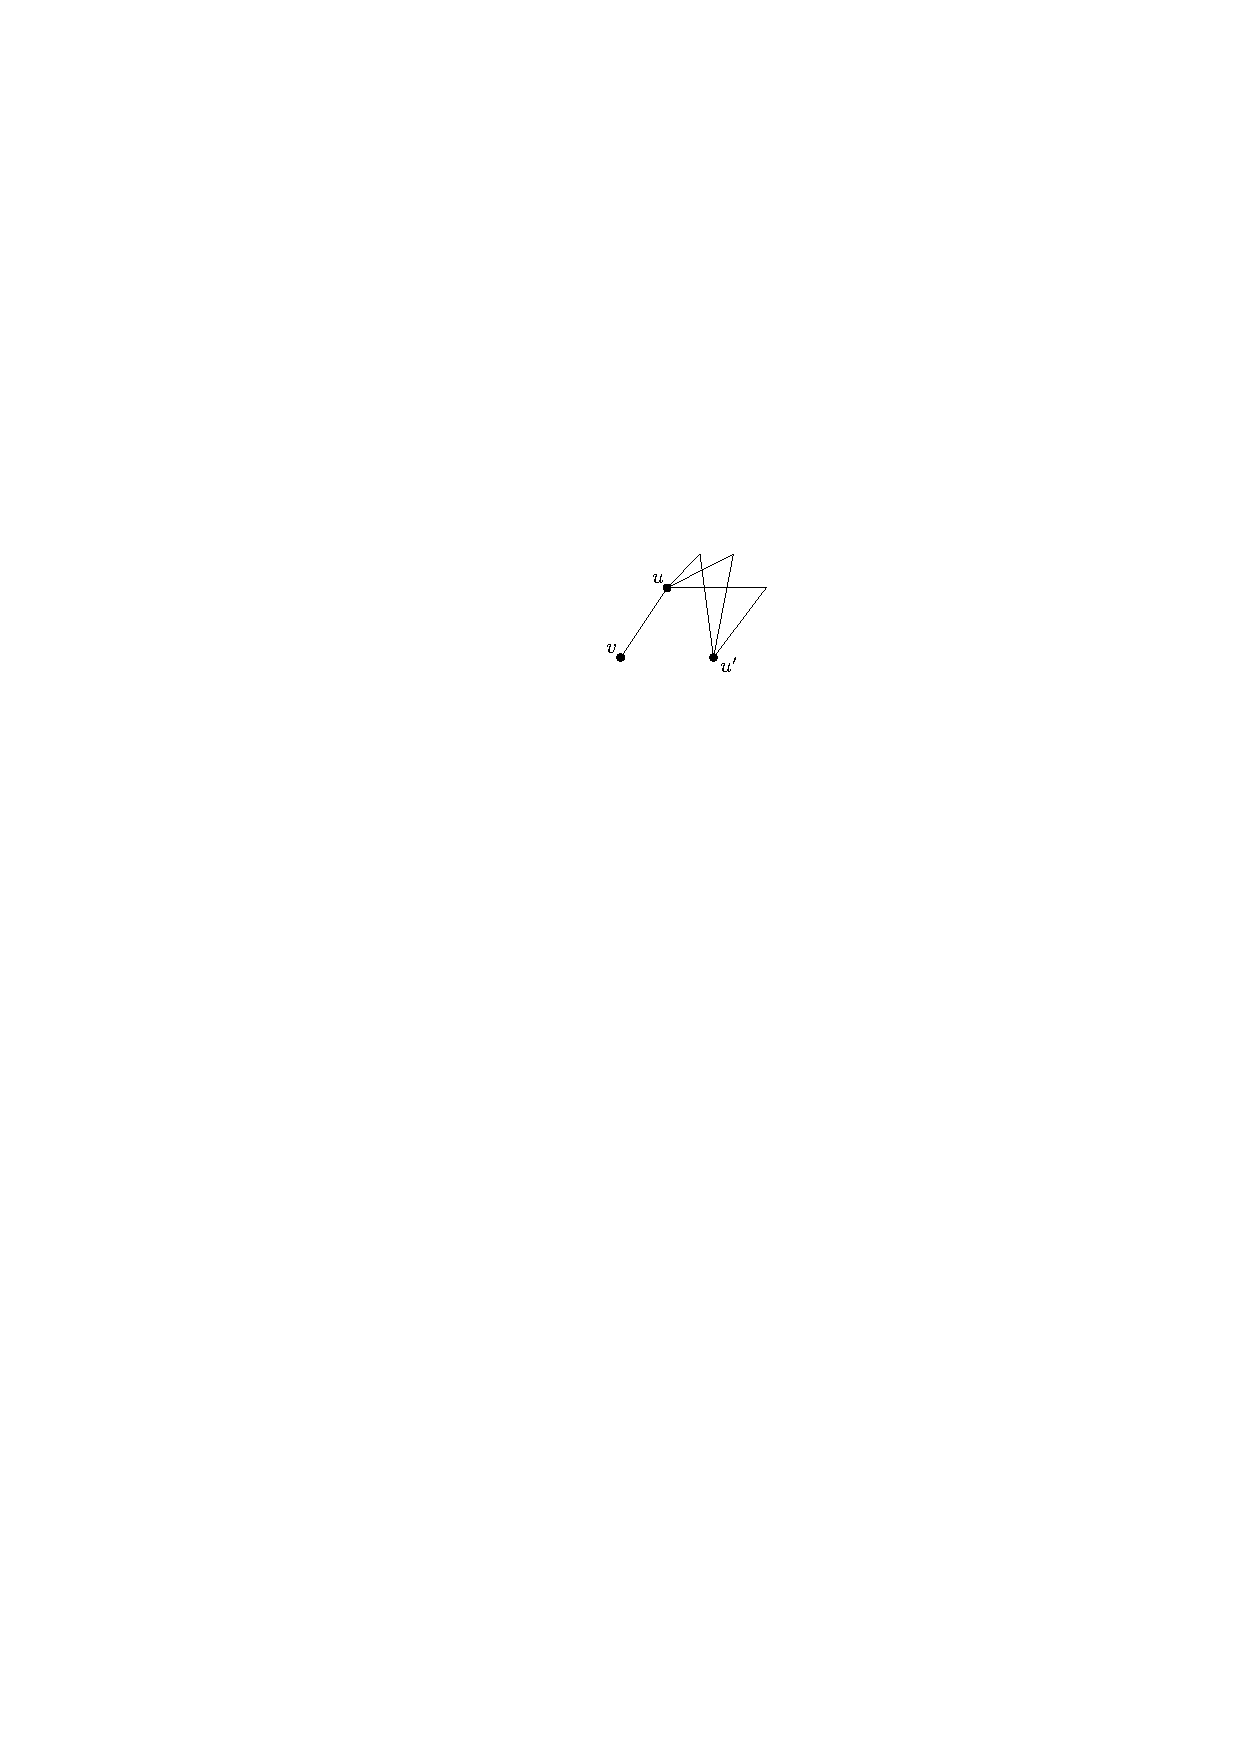
\includegraphics[width=3cm]{img/turan2.pdf}
\end{subfigure}
\caption{$d(w) < d(u)$}
\end{subfigure}
\hfill
\begin{subfigure}{8cm}
\begin{subfigure}{3cm}
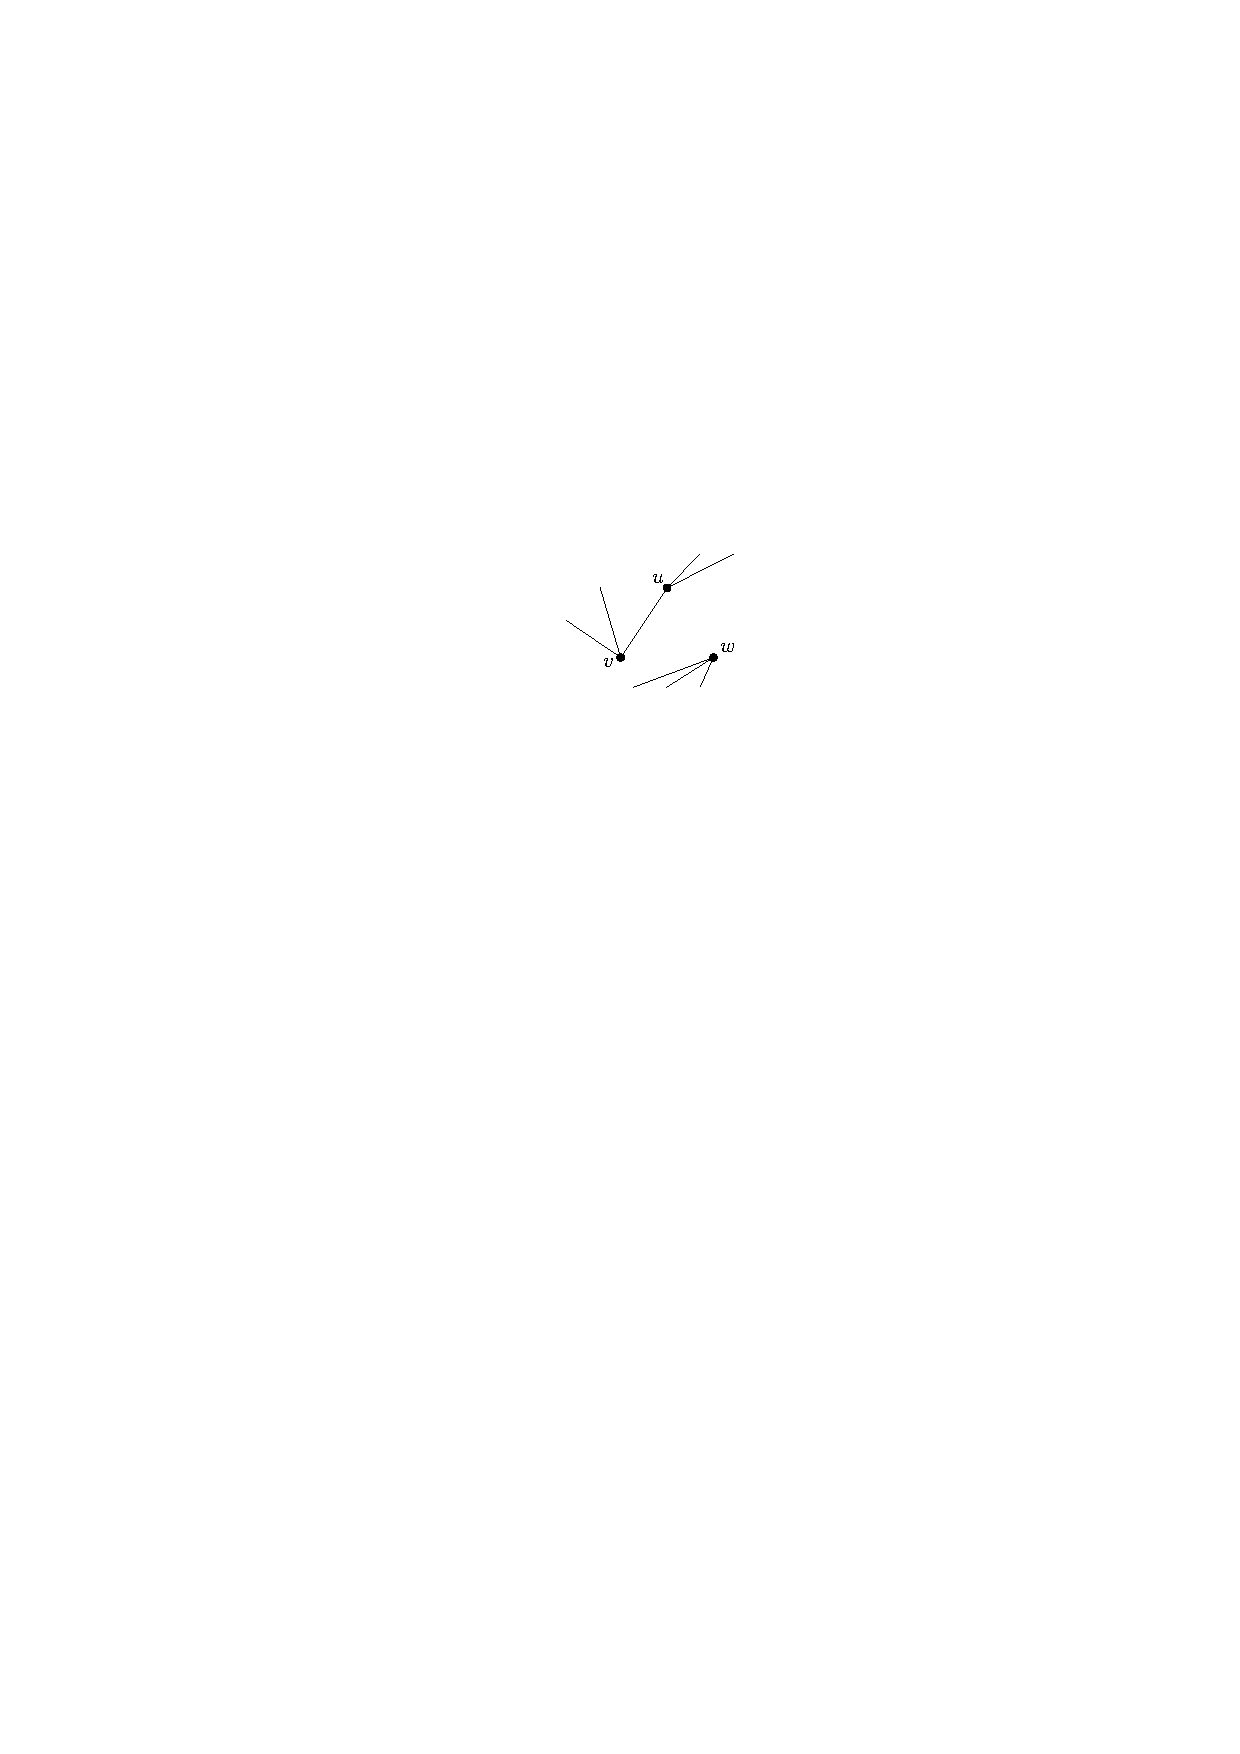
\includegraphics[width=3cm]{img/turan3.pdf}
\end{subfigure}
\hspace{0.5cm}$\Rightarrow$\hspace{0.5cm}
\begin{subfigure}{3cm}
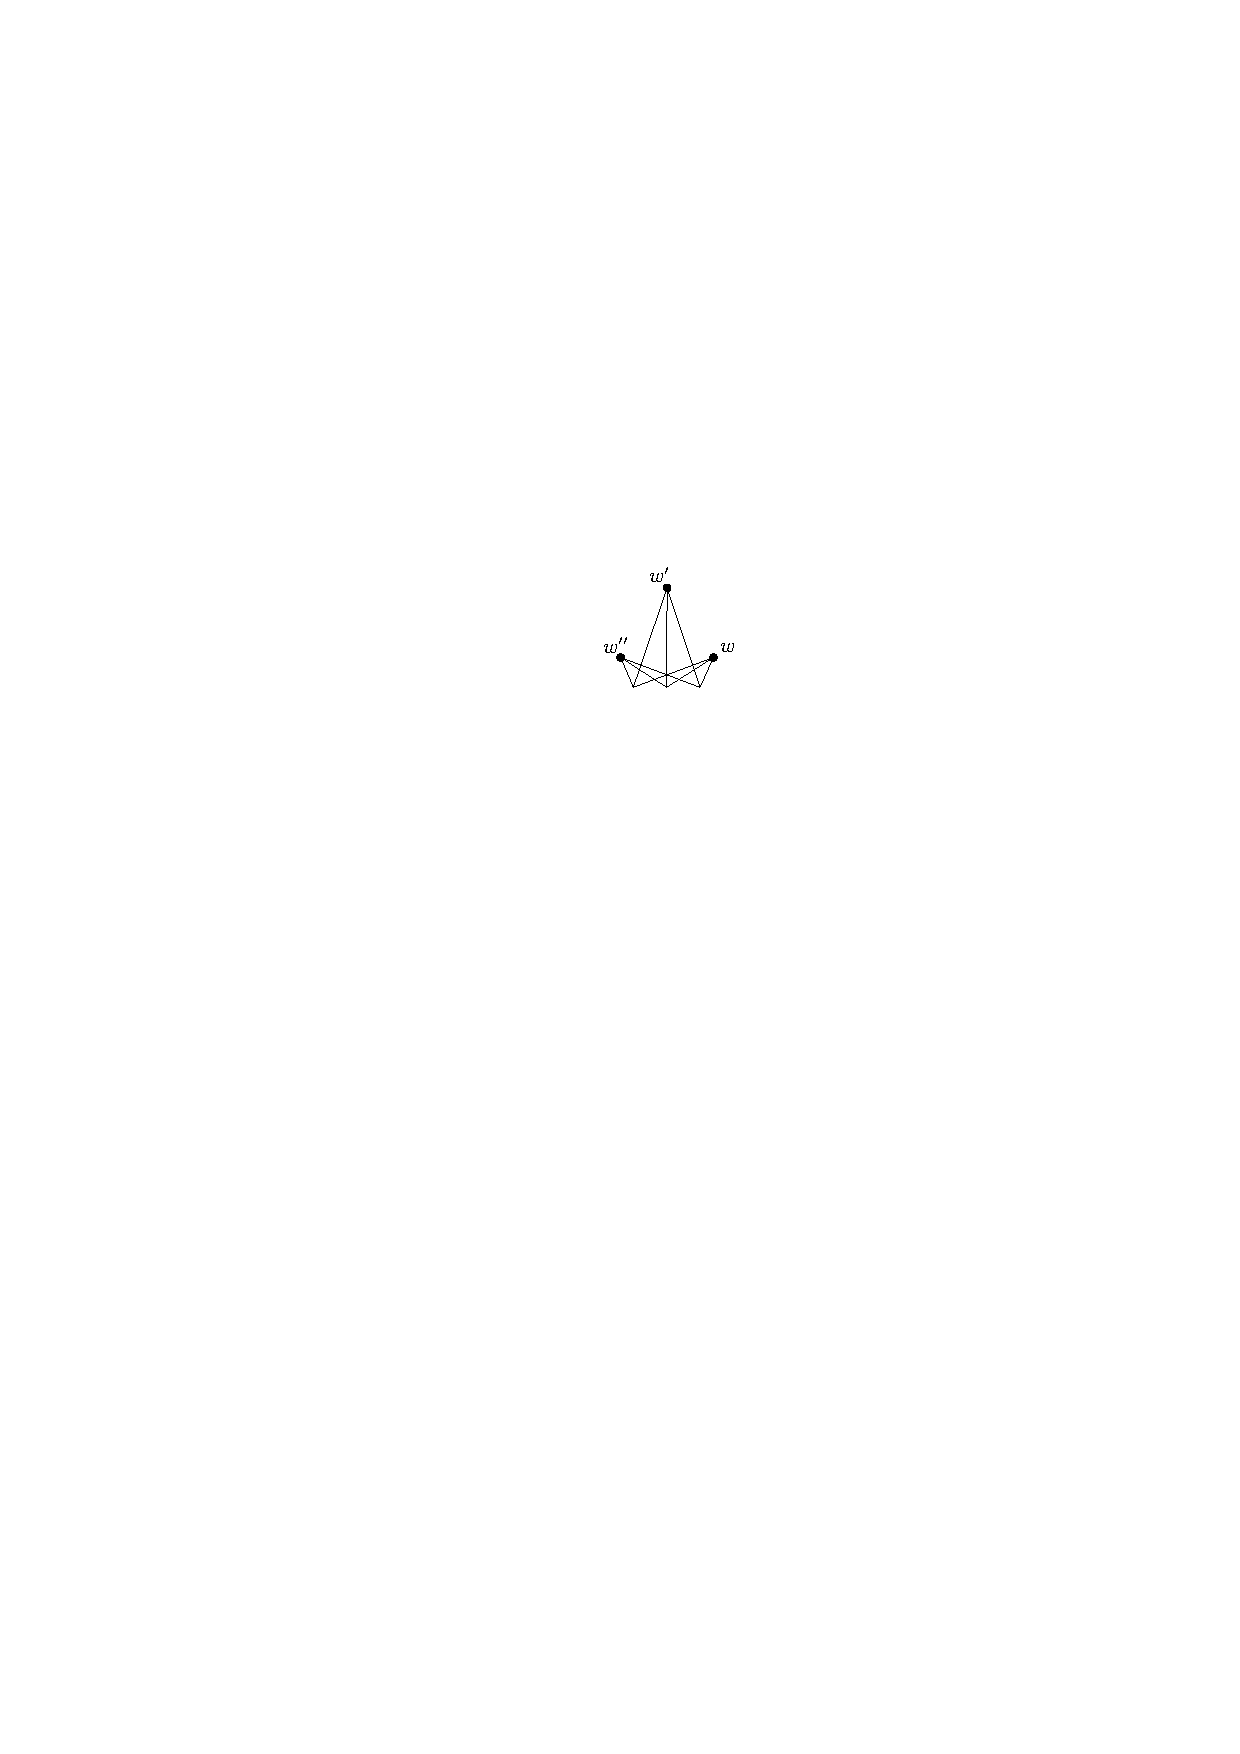
\includegraphics[width=3cm]{img/turan4.pdf}
\end{subfigure}
\caption{$d(w) \ge d(u)$ a $d(w) \ge d(v)$}
\end{subfigure}
\caption{Důkaz Turánovy věty, část 1.}
\end{figure}

\textbf{Část 2.} Mějme partity $A$ a $B$ tž. $|A| > |B| + 1$. Pak přesunem
vrcholu z $A$ do $B$ ztratíme $|B|$ hran, ale získáme $|A|-1$ hran a tedy
zvýšíme počet hran v $G$ alespoň o 1. Tedy, počet hran v $r$-partitním grafu je
maximální, když se velikosti partit liší nejvýše o 1.
\qed

\subsection{Ramseyovy věty}

\vt (Ramsey) {\it Pro každé $k \in \N$ existuje $n \in \N$ tž. každý graf na alespoň $n$ vrcholech obsahuje $K_k$ nebo indukovaný $\overline{K_k}$ jako podgraf.\footnote{Nejmenší takové $n$ pro dané $k$ nazýváme Ramseyovo číslo a značíme $R(k)$.}\footnote{Můžeme se setkat i s verzí, kdy určujeme velikost kliky a velikost nezávislé množiny zvlášť. Pak značíme Ramseyovo číslo $R(k,l)$.}}

\vt (Ramsey, vícebarevná) {\it Pro každé $t$ a $k$ existuje $N$ takové, že pro každou funkci $c: {[n]\choose 2} \rightarrow [t], n\geq N$ existuje množina $A \in {[n]\choose k}$, pro níž je funkce $c$ na $A\choose 2$ konstantní.} Jinými slovy, existuje dostatečně velké $N$ takové, že každý úplný graf alespoň na $N$ vrcholech obarvený $t$ barvami obsahuje jednobarevnou kliku velikosti $k$.

\vt (Ramsey, nekonečná) {\it Pro každé $t$ a každou funkci $c: {\N\choose 2} \rightarrow [t]$ existuje nekonečná množina $A\subseteq \N$, pro níž je funkce $c$ na $A\choose 2$ konstantní.} Neboli, v každém nekonečném úplném grafu obarveném $t$ barvami existuje nekonečně velká monochromatická klika.

\dk Sestrojíme si nekonečnou posloupnost nekonečných množin $A_1, A_2, \dots$ Začneme s $A_1 = \N$. Z $A_i$ zkonstruujeme $A_{i+1}$ tak, že si vybereme nejmenší prvek\footnote{Mohl by být libovolný, ale takhle se elegantně vyhneme problému s axiomem výběru.} $v_i \in A_i$ a rozdělíme vrcholy $A_i \setminus \{v_i\}$ na třídy ekvivalence $B_i^1, \dots, B_i^t$ podle toho, jakou barvu má hrana, která je spojuje s $v_i$. Podle nekonečného principu holubníku je alespoň jedna z $B_i^j$ nekonečná. Položme $b_i = j$ a $A_{i+1} = B_i^j$ a pokračujme dalším krokem (do nekonečna).

Všimněme si, že v posloupnosti vybraných vrcholů $(v_i)$ platí $\forall i < j$ má hrana $v_iv_j$ barvu $b_i$ (tedy záleží pouze na vrcholu s nižším pořadovým číslem). V nekonečné posloupnosti $b_1,b_2,\dots$ se musí některá z $t$ barev opakovat nekonečněkrát -- odpovídající vrcholy pak tvoří jednobarevný nekonečný úplný graf.
\qed

Konečná verze se dokazuje obdobně, ale musíme pečlivěji upočítat potřebnou velikost počáteční množiny.

\subsection{Hales-Jewett}

Zjednodušeně řečeno, Hales-Jewettova věta praví, že když dostanu od protivníka délku hrany krychle $a$ a počet barev $r$, dokážu najít dostatečně velkou dimenzi $N$, aby každé obarvení $N$-dimenzionální krychle o hraně $a$ pomocí $r$ barev obsahovalo jednobarevnou piškvorku délky $a$. Dále budeme značit $A = \{1, \dots, a\}$.

\vt (Hales-Jewett) {\it Pro každé $a$ (délka hrany krychle) a $r$ (počet barev) existuje $N = HJ(r,a)$ tž. obarvíme-li body krychle $A^N$ pomocí $r$ barev, vždy existuje jednobarevná kombinatorická přímka.}

\tv (o vnořené konzistentní krychli) {\it Existuje $N$ takové, že pro každé obarvení $\chi: A^N \rightarrow {1,\dots, r}$ existuje podkrychle $\alpha[A^n] \subset A^N$ obarvená konzistentně.} Konzistentně obarvená krychle znamená, že barvy na vnější slupce (bodech, jejichž nějaká souřadnice je 0) jsou kopiemi barev sousedních vrcholů o jednu vrstvu hlouběji.

\dk \textbf{(Idea)} Zafixujeme si $r$ a důkaz provedeme indukcí podle $a$. Pro $a=1$ je situace triviální. Pro větší $a$ použijeme pomocné tvrzení o vnořené konzistentní krychli a najdeme krychli $A^n$. Z té sloupneme vnější slupku, v krychli s o jedna kratší hranou nalezneme piškvorku (z indukčního předpokladu) a po doplnění slupky dostaneme piškvorku v $A^n$ (protože krychle je konzistentní). Piškvorka v $A^n$ je i piškvorkou v $A^N$ (jedná se o vnoření), čímž je indukční krok hotový.
\qed

Důkaz pomocného tvrzení je technický, takže jen uvedeme konstrukci $N$, abychom měli představu o jeho velikosti. Zadefinujeme $N = N_1 + \dots + N_n$, kde:

$$N_1 = r^{a^n},\qquad N_i = r^{a^{\left(n+\sum_{j=1}^{i-1} N_j\right)}}$$

\subsection{Van der Waerden}

\vt (Van der Waerden) {\it Pro každé $r, k \in \Z^+$ existuje $N$ takové, že v každém obarvení posloupnosti ${1, 2, \dots, N}$ $r$ barvami najdeme jednobarevnou aritmetickou posloupnost délky alespoň $k$.}

V praxi je takové $N$ obludně velké, nejlepší známý horní odhad tvrdí $W(r,k) \le 2^{2^{r^{2^{2^{k+9}}}}}$.

\dk Použijeme Hales-Jewetta a najdeme $N = HJ(r,k)$. Každé číslo $a \in \{0, 1, \dots, t^N-1\}$ můžeme zapsat v soustavě o základu $t$ jako $(a_0,a_1,\dots,a_{N-1})$, kde $a = a_0 + a_1t + \dots + a_{N-1}t^{N-1}$. Tím jsme získali bijekci mezi čísly od 0 do $t^N-1$ a vrcholy $N$-dimenzionální krychle o hraně $k$. Z Hales-Jewetta víme, že v krychli existuje kombinatorická přímka délky $k$. Kombinatorická přímka odpovídá aritmetické posloupnosti -- jedna její souřadnice nabývá hodnot od 0 do $N-1$ a všechny ostatní zůstávají konstantní.
\qed

